\chapter{Testing}

	The following describes how the product is tested.

	\section{Alpha Testing}
		\subsection{Function Testing}

		During function testing, each part of the system was tested individually.
		The following are some examples of function testing performed:
		\begin{itemize}
			\item Graphical input from camera
			\item Corresponding OCR input and output
			\item Summary feedback to user
		\end{itemize}

		\subsection{System Testing}

		The system was tested as a whole. The test is focused on where all modules and functions within the system are cooperating with each other, and whether the system functions as a whole.
		
		\subsubsection{Performance}
		The performance of the system is tested with a test set of 30 images (see Figure~\ref{testImages}) with both versions of Tesseract OCR – Tesseract 3.05.00 \cite{tesseract3} and Tesseract 4.00.00 \cite{tesseract4}.
		
		The test results (see Table~\ref{performanceAnalysis}) show that Tesseract 4 provides significant better results than Tesseract 3, even though Tesseract 4 is still in alpha stage.
		
		The documents in the test images are collected from BBC News (www.bbc.com). This way the ground truth of the document (the original computer encoded characters) can be used to compare with the result of the system.
		
The test images cover a variety of different backgrounds, motions, blurriness and brightness. 
		
\begin{figure}
  \begin{subfigure}{\linewidth}
  	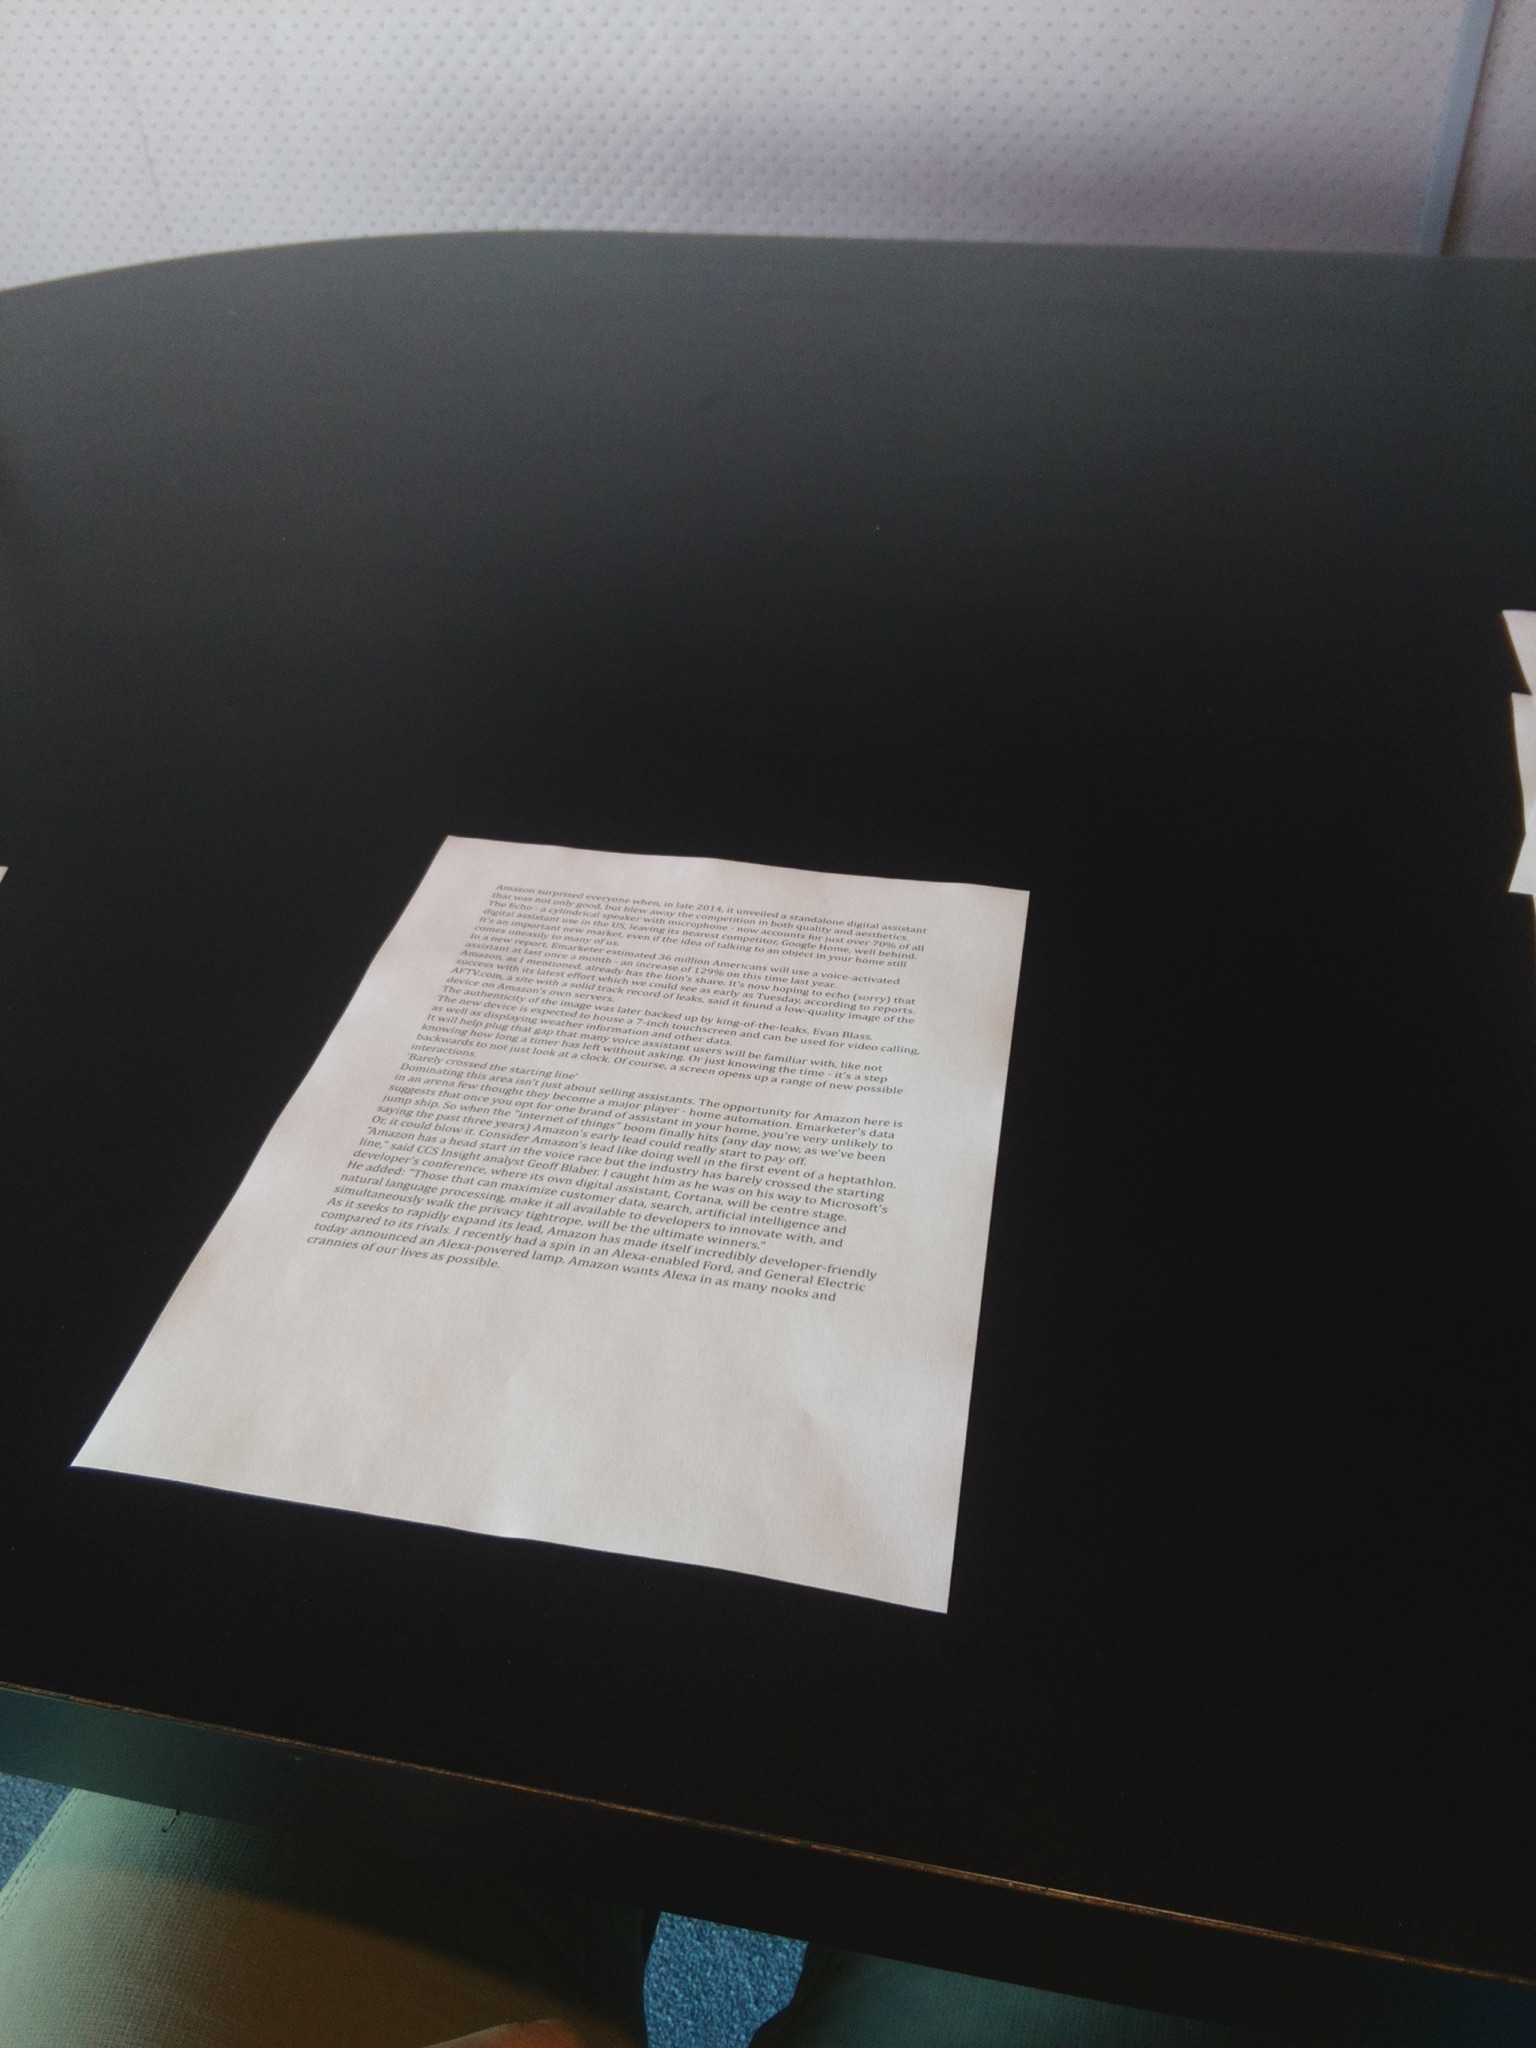
\includegraphics[width=.24\linewidth]{Amazon.jpeg}\hfill
	  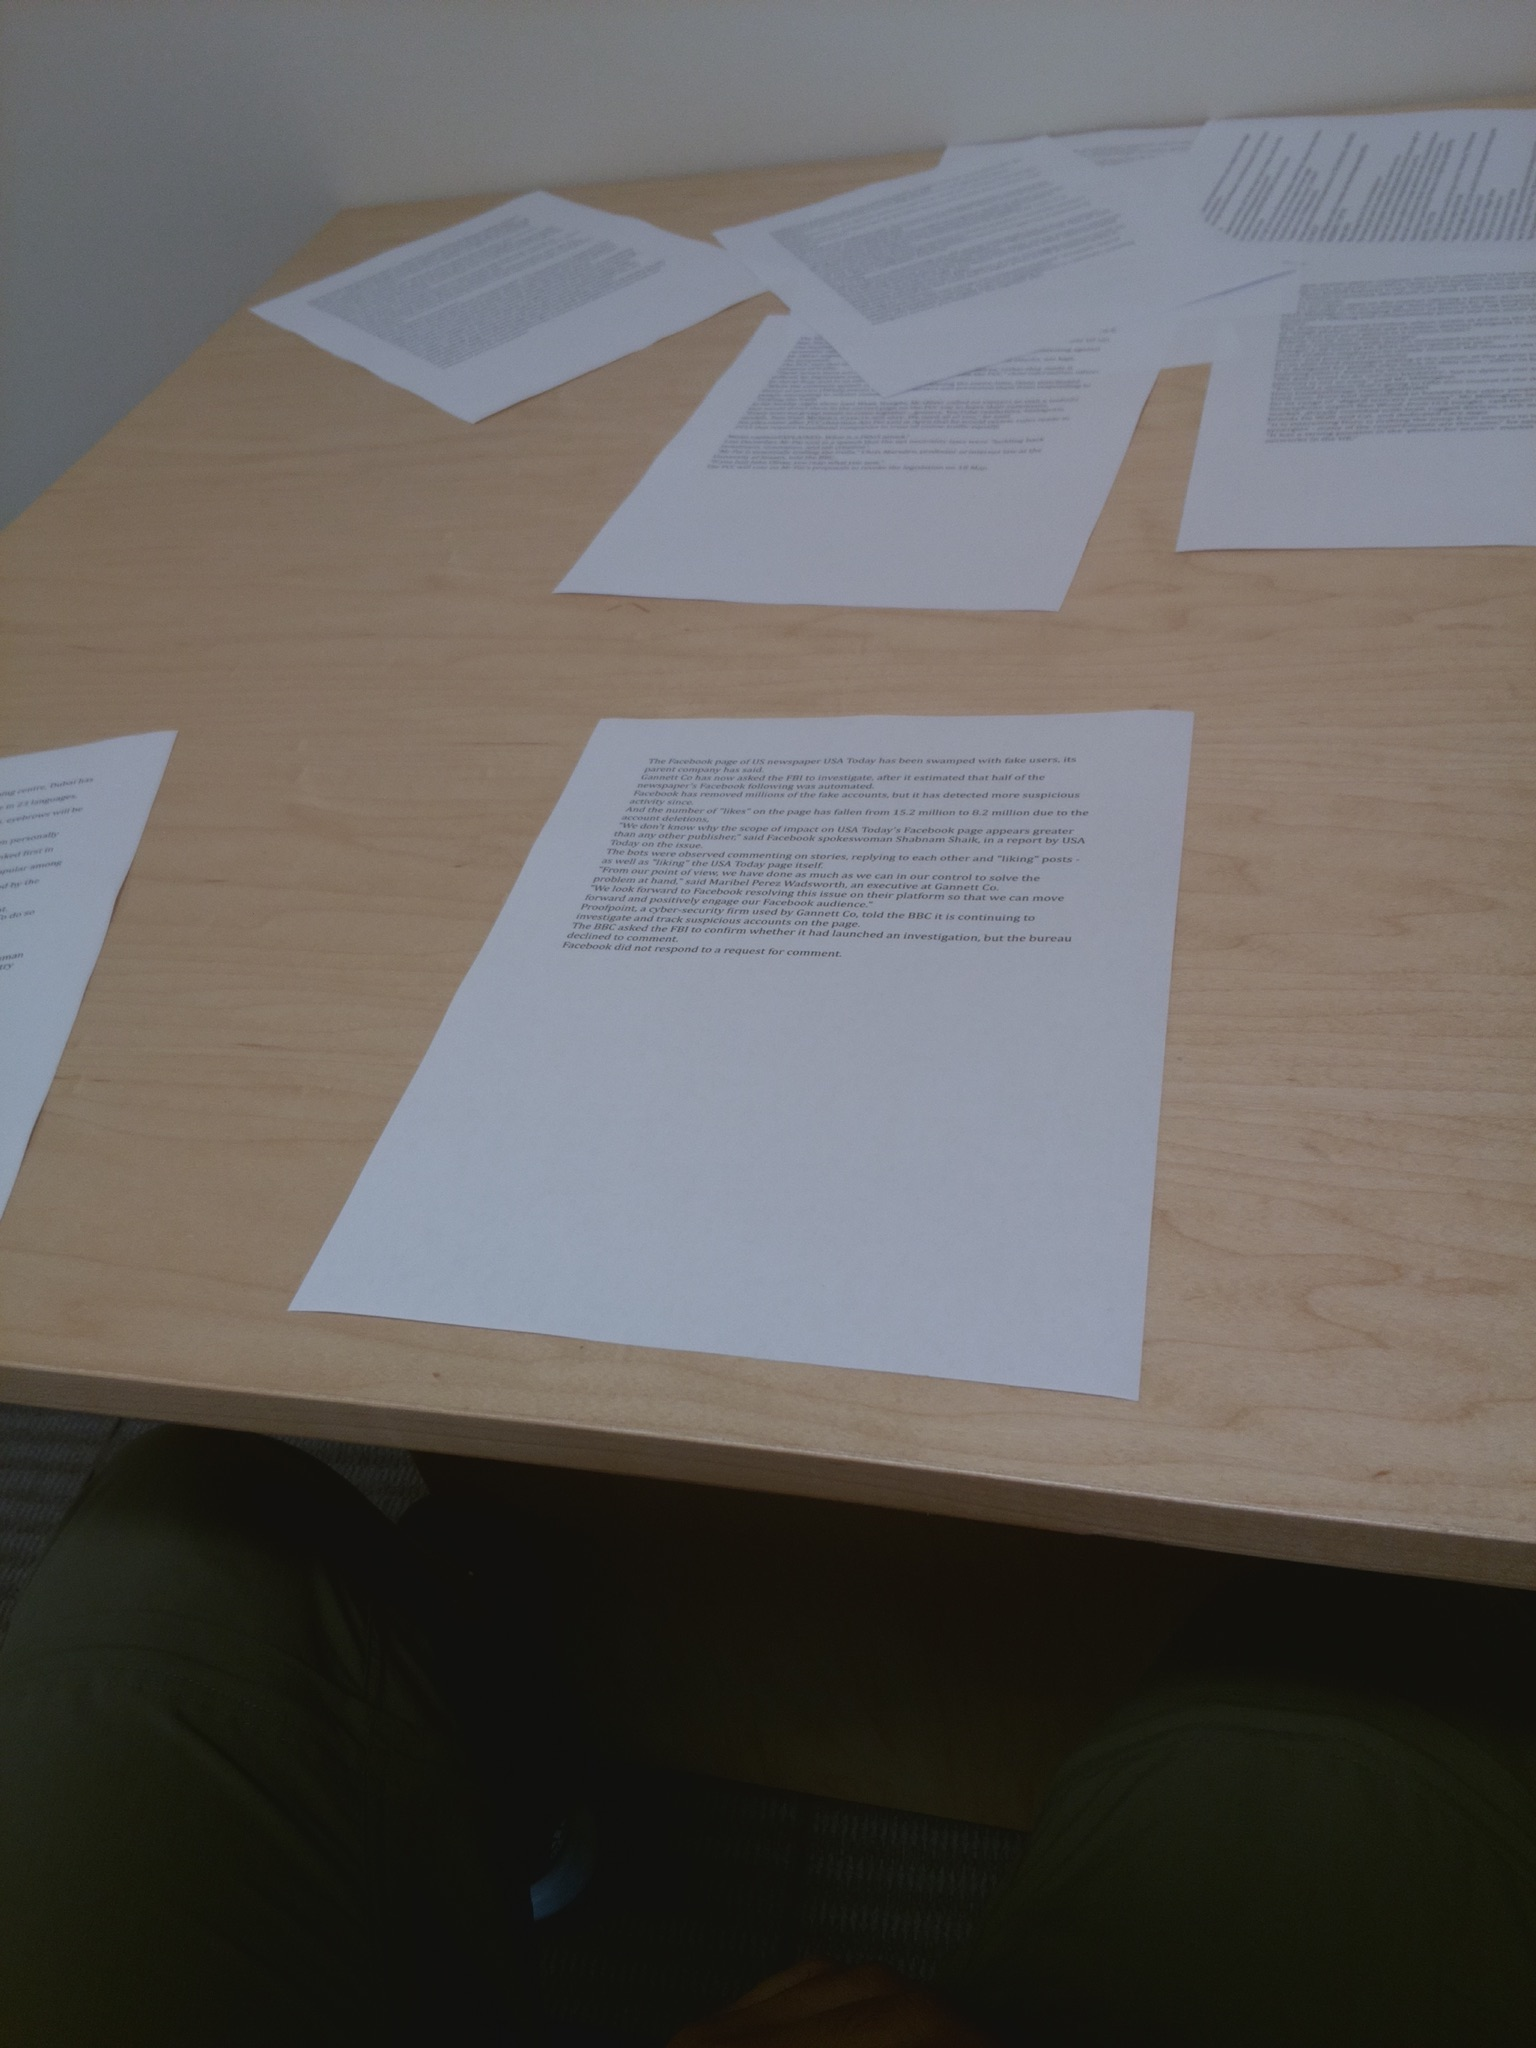
\includegraphics[width=.24\linewidth]{FacebookBot.jpeg}\hfill
	  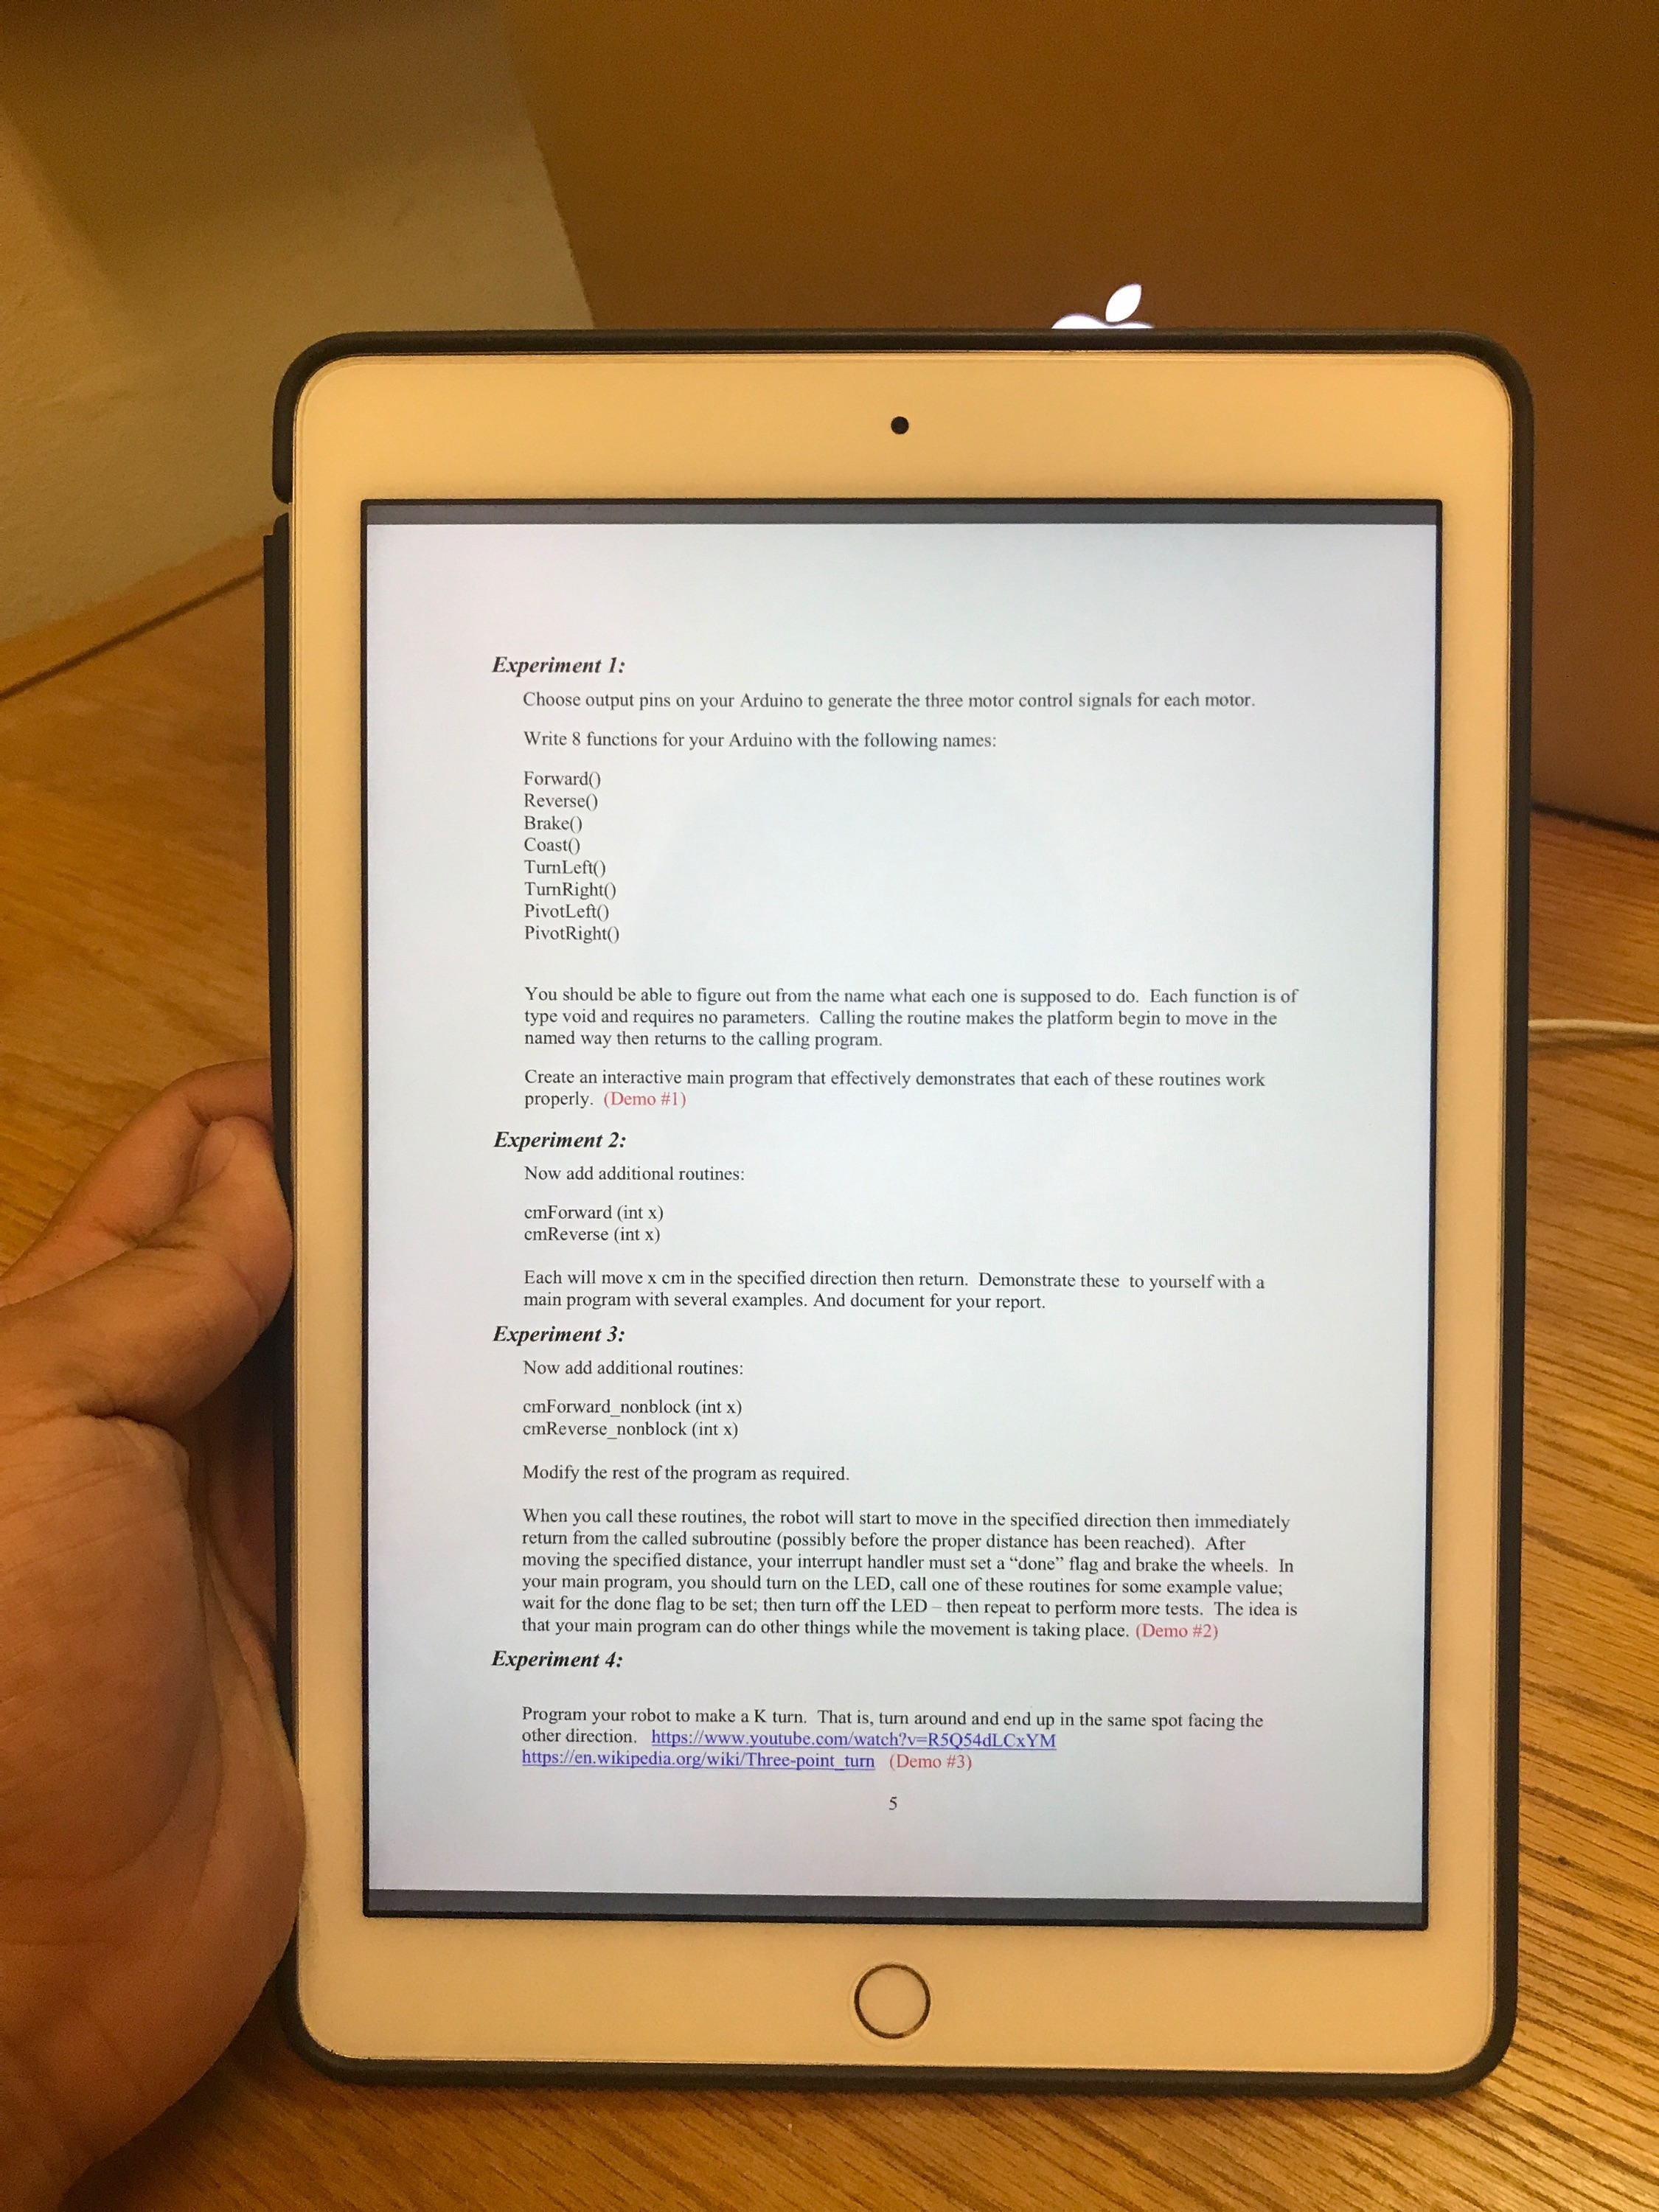
\includegraphics[width=.24\linewidth]{IMG_9203.jpeg}\hfill
	  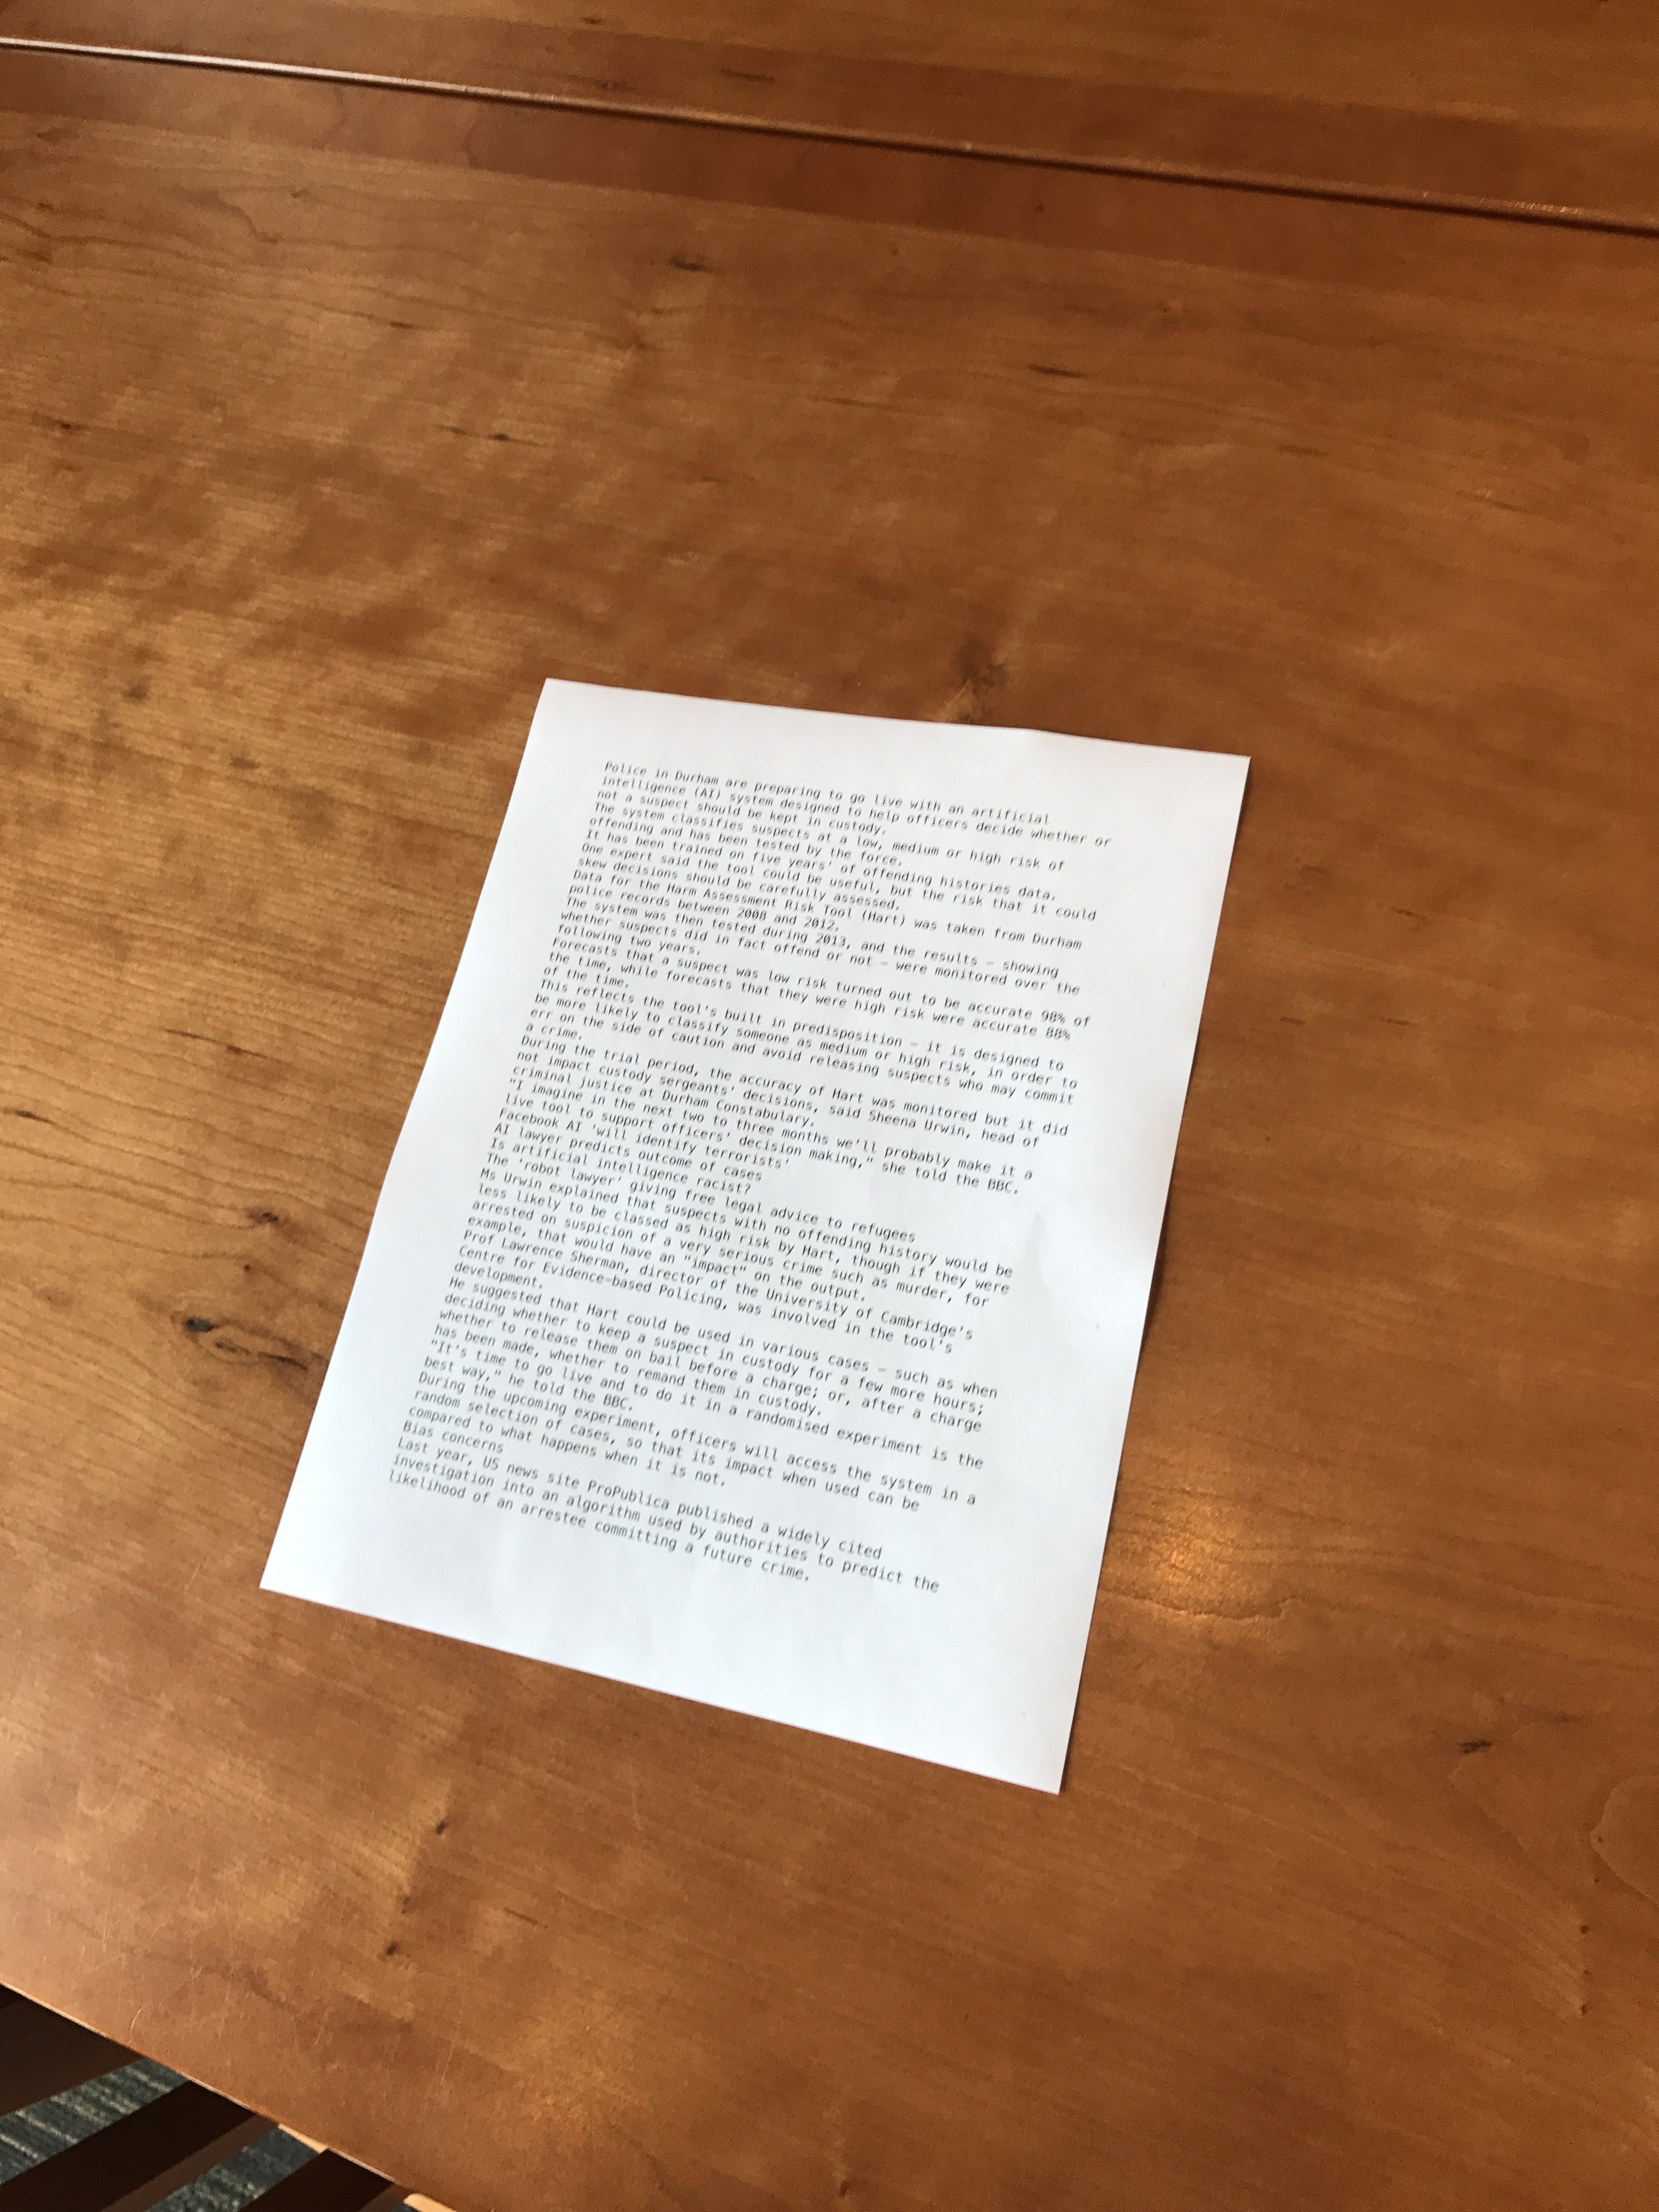
\includegraphics[width=.24\linewidth]{IMG_9259.JPG}
  \end{subfigure}\par\medskip  
  
  \caption{Testing images gathered during System Testing}
  \label{testImages}
\end{figure}


		
\begin{table}[]
\centering
\caption{Performance Analysis}
\label{performanceAnalysis}
\begin{tabular}{l|l|l|l|l|}
\cline{2-5}
\multirow{2}{*}{}                          & \multicolumn{2}{c|}{\textbf{Accuracy (\%)}} & \multicolumn{2}{c|}{\textbf{Response Time (Sec)}} \\ \cline{2-5} 
                                           & Mean           & Standard Deviation         & Mean              & Standard Deviation            \\ \hline
\multicolumn{1}{|l|}{\textbf{Tesseract 3}} & 35.93          & 21.37                      & 11.05             & 4.68                          \\ \hline
\multicolumn{1}{|l|}{\textbf{Tesseract 4}} & 91.07          & 7.24                       & 3.07              & 0.60                          \\ \hline
\end{tabular}
\end{table}